\section{Results}
\label{sec:results}

\subsection{Phrases are recovered several tokens ahead}
\label{sec:lookahead}

\begin{table}[t]
\centering\small
\begin{tabular}{lrrrr}
\toprule
& \multicolumn{4}{c}{\textbf{Lookahead distance} $i$} \\
\cmidrule(lr){2-5}
\textbf{Readout / condition} & 2 & 3 & 4 & 5 \\
\midrule
\multicolumn{5}{l}{\textit{Phrase in isolation}} \\
\quad Patchscopes & 57.8 & 30.9 & 19.4 & 16.5 \\
\quad Generation & 59.2 & 31.2 & 20.6 & 17.6 \\
\midrule
\multicolumn{5}{l}{\textit{Phrase in natural context}} \\
\quad Patchscopes & 73.2 & 57.5 & 43.9 & 38.7 \\
\quad Generation & 84.0 & 64.8 & 55.6 & 53.6 \\
\midrule
\multicolumn{5}{l}{\textit{Robustness: wider Patchscopes layer sweep}} \\
\quad Patchscopes, all 32 layers & 79.6 & 64.1 & 51.6 & 46.4 \\
\bottomrule
\end{tabular}
\caption{Recovery rate (\%) of the final $i$ phrase tokens, OLMo-2-7B.
Isolation rows are computed over phrases
(1,112 at $i=2$); context rows over
(phrase, context) instances (9,148,
8,529,
4,677 and
2,386 at $i=2\ldots5$).
Patchscopes counts a success if \emph{any} probed layer recovers the
continuation, over the eight layers used throughout this paper
(\S\ref{sec:setup}); isolation rows sweep all 32. The final row re-runs the
in-context sweep over all 32 layers and is discussed in
\S\ref{sec:disagreement}.}
\label{tab:main}
\end{table}


\begin{figure}[t]
\centering
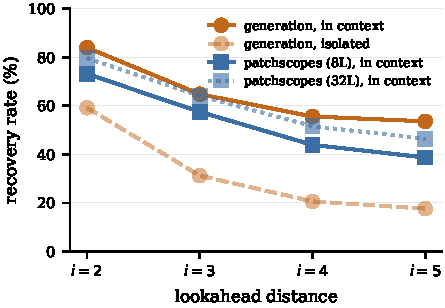
\includegraphics[width=\columnwidth]{figures/context_vs_isolation}
\caption{Recovery rate against lookahead distance. Natural context lifts the
generation readout by $25$--$36$ points over the same phrases in isolation. The
two Patchscopes curves are the same measurement under different layer budgets
and differ by $6$--$8$ points, which is most of the apparent gap to generation
(\S\ref{sec:disagreement}).}
\label{fig:context}
\end{figure}

Table~\ref{tab:main} gives the central measurement. In natural context,
OLMo-2-7B completes a familiar phrase two tokens early in $84.0\%$ of instances,
three tokens early in $64.8\%$, and five tokens early in $53.6\%$. Anticipation
of fixed expressions is therefore not a marginal effect at short range; it
persists at distances of several tokens, well past the horizon of ordinary
next-token prediction.

\paragraph{Isolation understates the effect.}
The same phrases presented alone, with no surrounding text, are recovered far
less often: $59.2\%$ at $i=2$ falling to $17.6\%$ at $i=5$ (Figure~\ref{fig:context}).
The gap widens with distance, from $24.8$ points at $i=2$ to $36.0$ points at
$i=5$, and the Patchscopes readout shows the same pattern. This is the expected
direction --- context supplies both topical evidence and the signal that a fixed
expression is under way --- but its size matters for interpreting prior
results. A bare phrase is a poor proxy for the condition
under which a model actually encounters these expressions, and measurements
taken in isolation should be read as a lower bound.

\paragraph{Successes persist beyond the range we analyse.}
We restrict the main analysis to $i \leq 5$ because instance counts fall
steeply beyond that. The effect does not stop there, however: in context,
generation recovers $48.9\%$ of the $1{,}123$ trials at $i=6$ and $41.7\%$ of
the $312$ at $i=8$. We do not draw conclusions from the sparse tail, but we note
it because an earlier version of this work reported zero successes at
$i \geq 6$; that was an artifact of a fixed generation budget
(\S\ref{sec:criterion}), not a property of the model.

\subsection{Anticipation is a property of the phrase}
\label{sec:stability}

\begin{figure}[t]
\centering
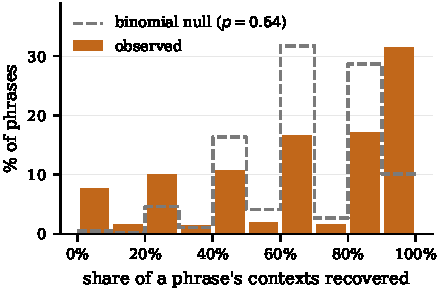
\includegraphics[width=\columnwidth]{figures/per_phrase_consistency}
\caption{Share of its own distinct contexts in which each phrase's continuation
is recovered at $i=3$, generation readout, over the $803$ phrases with at least
five distinct contexts. The dashed line is the binomial distribution expected if
every context were an independent draw at the pooled rate $p=0.64$. The observed
distribution puts mass at both extremes, where the null has almost none.}
\label{fig:consistency}
\end{figure}

An aggregate rate of $64.8\%$ at $i=3$ is consistent with two very different
pictures. Either the model recovers most phrases most of the time with some
per-occasion noise, or it reliably recovers some phrases and reliably fails on
others. Only the second supports the idea of a stable, reusable phrase-level
representation.

For each of the $803$ phrases with at least five distinct contexts
(\S\ref{sec:setup}) we compute the share of its contexts that succeed, and
compare the resulting distribution against the binomial null in which every
context is an independent draw at the pooled rate $p = 0.645$
(Figure~\ref{fig:consistency}). The two differ sharply. $31.5\%$ of phrases
succeed in at least $90\%$ of their contexts where the null predicts $10.1\%$,
and $18.3\%$ succeed in at most $20\%$ where the null predicts $5.0\%$;
conversely only $27.3\%$ fall in the $40$--$60\%$ band that holds $48.5\%$ of
the null's mass. The Patchscopes readout is more extreme still, at $37.4\%$ and
$22.5\%$ against nulls of $9.5\%$ and $5.4\%$.

We read this as evidence that what varies is the phrase, not the occasion. Some
expressions are reliably available to the model ahead of time and others are
reliably not, and context modulates that availability rather than creating it.
This is what makes the probing question in \S\ref{sec:probe} worth asking: a
signal that is stable per phrase is a signal that something in the
representation could carry.

\subsection{Where in the model the phrase becomes readable}
\label{sec:layers}

\begin{figure}[t]
\centering
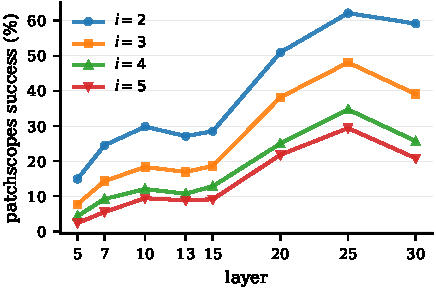
\includegraphics[width=\columnwidth]{figures/patchscopes_by_layer}
\caption{Patchscopes success by layer and lookahead distance, in context, over
the eight probed layers. Recovery rises through the network, peaks at L25, and
falls at L30 at every distance.}
\label{fig:bylayer}
\end{figure}

Recording Patchscopes success separately at each of the eight probed layers
(Figure~\ref{fig:bylayer}) gives a consistent shape across all four distances:
recovery is low in the early layers, rises through the middle of the network,
peaks at L25 --- $62.2\%$ at $i=2$, $48.1\%$ at $i=3$ --- and then falls back at
L30, to $59.2\%$ and $39.1\%$. The decline in the last layers appears at every
$i$ and in every category.

One explanation is that the final layers specialise toward producing the actual
next token for the real input rather than maintaining a general, transferable
representation, so a state lifted from L30 and pasted into an unrelated prompt
transfers less well than one lifted from L25. We note that this is a hypothesis
consistent with our data and with the late-layer decline reported by
\citet{kaplan-etal-2025-tokens} for word-level retrieval, not something these
experiments establish; a state that a patchscope can no longer verbalise may
still carry the information in a form the rest of the network can use.

Taking the union over all $32$ layers rather than eight, the median first
successful layer is L16, and $41.9\%$ of successes first appear at or before
L10 (Appendix~\ref{app:details}). Phrase information thus becomes readable
gradually and, for a large minority of cases, quite early.

\subsection{The two readouts disagree}
\label{sec:disagreement}

\begin{table}[t]
\centering\small
\begin{tabular}{rrrrrrr}
\toprule
$i$ & $n$ & both & \makecell{ps.\\only} & \makecell{gen.\\only} & neither & \makecell{agree\\(\%)} \\
\midrule
2 & 9,148 & 6,757 & 521 & 923 & 947 & 84.2 \\
3 & 8,529 & 4,681 & 783 & 849 & 2,216 & 80.9 \\
4 & 4,677 & 1,968 & 445 & 632 & 1,632 & 77.0 \\
5 & 2,386 & 933 & 175 & 347 & 931 & 78.1 \\
\midrule
2--5 & 24,740 & 14,339 & 1,924 & 2,751 & 5,726 & 81.1 \\
\bottomrule
\end{tabular}
\caption{Patchscopes (32-layer union) and generation on \emph{identical}
(phrase, context, $i$) instances. The two readouts disagree on
18.9\% of instances, and the disagreement runs in both
directions: 1,924 instances are recovered only by
patchscopes and 2,751 only by generation.}
\label{tab:agreement}
\end{table}

\begin{table}[t]
\centering\small
\begin{tabular}{lrrr}
\toprule
& & \multicolumn{2}{c}{\textbf{Recovery (\%)}} \\
\cmidrule(lr){3-4}
\textbf{Category} & \textbf{Inst.} & patchscopes & generation \\
\midrule
Landmarks & 1,409 & 56.8 & 75.3 \\
Idioms & 20,371 & 65.9 & 66.4 \\
Film titles & 2,960 & 68.6 & 84.5 \\
\bottomrule
\end{tabular}
\caption{Recovery by phrase category, pooled over $i=2\ldots5$, in natural
context. The two readouts order the categories differently: under generation,
idioms are the hardest category, while under patchscopes they sit between
landmarks and film titles.}
\label{tab:categories}
\end{table}


So far we have reported both readouts as if they were interchangeable
measurements of one underlying quantity. They are not. Table~\ref{tab:agreement}
compares them on identical instances --- same phrase, same context, same cut
point, same success criterion --- and they agree on $78.7\%$ of the $24{,}740$
pooled trials.

The residual $21.3\%$ is the informative part. It is lopsided: generation
recovers a continuation that Patchscopes misses in $15.7\%$ of instances, while
Patchscopes recovers one that generation misses in only $5.6\%$ --- roughly a
three-to-one asymmetry. Read on its own, that says Patchscopes undercounts what
the model can do.

But the two failure directions are qualitatively different, and neither is
simply an instrument defect. Where Patchscopes succeeds and generation does not,
the state does contain the phrase --- the patchscope verbalises it --- yet the
real context steers the model elsewhere; given \textit{Why should one person be
brought up}, the model writes \textit{a wealthy family, with every opportunity}
instead of completing \textit{in the lap of luxury}. Where generation succeeds
and Patchscopes does not, the model completes the phrase correctly from its real
prefix while the patchscope, at the same position, reaches for a neighbouring
expression: for \textit{a bird in the hand is worth two in the bush} it returns
\textit{worth more than one}. The first is a continuation that was available but
not taken; the second is a readout that recovered the sense and lost the
wording.

\paragraph{The asymmetry is partly a layer-budget artifact.}
The comparison above gives Patchscopes eight layers. Sweeping all $32$ raises
its in-context rate from $73.2\%$ to $79.6\%$ at $i=2$ and from $38.7\%$ to
$46.4\%$ at $i=5$ (Table~\ref{tab:main}), lifts agreement to $81.1\%$, and
rebalances the disagreement from three-to-one to roughly three-to-two
(Table~\ref{tab:agreement}). At $i=3$ the two readouts then differ by $0.7$
points overall. Most of the apparent superiority of generation is therefore a
statement about how thoroughly Patchscopes was sampled, not about the model.
What survives the wider sweep is the disagreement itself: even at $32$ layers,
$18.9\%$ of instances are classified differently, and $7.8\%$ are recovered only
by Patchscopes. The two instruments are not nested, and no layer budget makes
one a refinement of the other.

We use the eight-layer readout as our primary measurement because it is the
layer set on which every per-layer, per-category and probing analysis in this
paper was run, so all of those results are mutually consistent. Readers
comparing our Patchscopes rates against other work should note that the budget
moves them by six to eight points.

\paragraph{Category difficulty is readout-dependent.}
Table~\ref{tab:categories} breaks the pooled rates down by phrase kind, and the
two readouts do not merely differ in level --- they reverse an ordering. Under
Patchscopes, idioms are the \emph{easiest} category at $57.4\%$, ahead of film
titles ($54.7\%$) and landmarks ($47.2\%$). Under generation, idioms are the
\emph{hardest} at $66.4\%$, well behind film titles ($84.5\%$) and landmarks
($75.3\%$). The reversal is consistent with the scoring artifact of
\S\ref{sec:falsepos}: idioms have accepted variants, so exact-match scoring
penalises them most under the readout that produces the most fluent
continuations. Under the wider $32$-layer sweep idioms move to the middle of the
Patchscopes ranking rather than the top, so the reversal weakens to a
re-ordering, but the categories are still ranked differently by the two
instruments.

The practical consequence is narrow but real. A study measuring only with
Patchscopes would report that this model handles idioms better than landmarks or
titles; one measuring only with generation would report the opposite. Both would
be reporting their instrument as much as their model.

\subsection{The hidden state predicts real completion}
\label{sec:probe}

\begin{table}[t]
\centering\small
\begin{tabular}{rrrrrr}
\toprule
& \multicolumn{3}{c}{\textbf{Patchscopes label}} & \multicolumn{2}{c}{\textbf{Generation label}} \\
\cmidrule(lr){2-4}\cmidrule(lr){5-6}
\textbf{Layer} & pos.\ (\%) & bal.\ acc. & prec. & bal.\ acc. & prec. \\
\midrule
5 & 6.6 & 76.0 & 33.9 & 69.8 & 83.3 \\
7 & 14.7 & 70.2 & 42.8 & 71.0 & 84.2 \\
10 & 18.8 & 76.5 & 52.3 & 72.0 & 84.9 \\
13 & 16.9 & 74.8 & 45.8 & 73.6 & 85.6 \\
15 & 18.5 & 76.3 & 51.1 & 74.2 & 86.1 \\
20 & 36.8 & 70.4 & 62.4 & 73.6 & 85.8 \\
25 & 47.7 & 68.1 & 67.2 & 74.6 & 86.2 \\
30 & 40.2 & 66.4 & 59.7 & 76.8 & 87.6 \\
\bottomrule
\end{tabular}
\caption{Probes trained on the hidden state at the cut position to predict each
readout's outcome, pooled over $i=2\ldots5$, split by phrase (80/20), training
set class-balanced by downsampling, evaluated on the natural test distribution.
The generation label has a fixed positive rate of 69.1\% at every
layer; the patchscopes label does not, which is why its raw accuracy is not
comparable across layers. Balanced accuracy for the patchscopes label peaks in
the middle of the model, whereas for the generation label it rises
monotonically with depth.}
\label{tab:probes}
\end{table}


\begin{figure}[t]
\centering
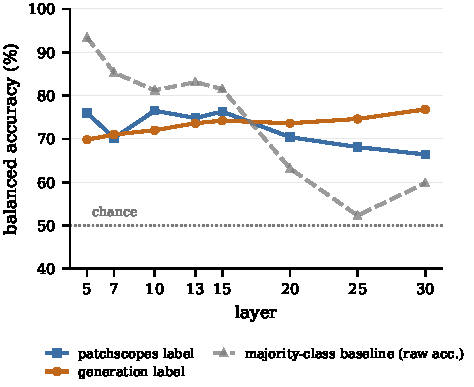
\includegraphics[width=\columnwidth]{figures/probe_balanced_accuracy}
\caption{Balanced accuracy of the two probes by layer. The label determines the
shape: predicting Patchscopes success peaks in the middle layers, while
predicting real completion rises monotonically to L30.}
\label{fig:probes}
\end{figure}

If phrase anticipation is carried by the representation, it should be readable
from the representation without an intervention. We train a small MLP
($32$ hidden units) on the raw hidden state at the cut position to predict, as a
binary label, whether the readout succeeds. Data are pooled over
$i \in \{2,3,4,5\}$ and split by phrase at $80/20$, so no test phrase appears in
training; the training set is class-balanced by downsampling and the test set is
left at its natural distribution.

Predicting \emph{real completion} works well. Balanced accuracy rises
monotonically with depth, from $69.8\%$ at L5 to $76.8\%$ at L30, and precision
is high and nearly flat at $83.3\%$ to $87.6\%$ (Table~\ref{tab:probes}). A
positive call from this probe is right roughly seven times in eight, and it is
made from a single hidden vector, before the model has produced any of the
tokens in question.

\paragraph{The signal is learned, not a base rate.}
Because $69.1\%$ of instances are positive, a probe could score respectably by
guessing. Two checks argue against that reading. First, balanced accuracy
corrects for the base rate by construction, and the probe clears $50\%$
everywhere. Second, running the same probe on the earliest layers gives a clean
gradient: $58.6\%$ balanced accuracy at L0 --- the raw embedding, before any
contextual processing --- rising to $65.1\%$ at L1, $66.5\%$ at L2 and $69.8\%$
at L5. A base-rate artifact would be flat across layers; this climbs as
computation accumulates. We note nonetheless that $58.6\%$ at L0 is above
chance, which suggests some of the signal is carried by lexical identity of the
cut token rather than by contextual processing.

\paragraph{The label changes where the ``best'' layer is.}
Training the identical architecture on the Patchscopes label instead produces a
different profile: balanced accuracy peaks in the middle of the network
($76.5\%$ at L10, $76.3\%$ at L15) and is worst at L30 ($66.4\%$), the mirror
image of the generation-label curve (Figure~\ref{fig:probes}). Raw accuracy for
this probe is not comparable across layers at all, because the positive rate
moves from $6.6\%$ at L5 to $47.7\%$ at L25 as Patchscopes itself gets better.
A reader interested in \emph{where in the model phrase information lives} would
draw opposite conclusions from the two probes. We read the generation-label
probe as the more trustworthy of the two, since its label does not depend on the
layer being probed, but the divergence is itself the point.

\subsection{Most apparent errors are valid alternates}
\label{sec:falsepos}

The probe's precision is bounded by the scoring criterion, not only by the
model. We adjudicated all $412$ false positives of the generation-label probe at
L25 --- cases where the probe predicted completion and exact-match scoring
recorded a failure --- using an LLM judge asked whether the generated text means
the same as the target. It labelled $62.9\%$ valid alternates,
$17.5\%$ partially correct and $19.7\%$ unrelated. Typical valid alternates are
\textit{laughs best} for \textit{laughs loudest}, \textit{plowshares} for
\textit{ploughshares}, and \textit{beat around the bush} for \textit{beat about
the bush}: the more common form of the expression, scored as a failure.

Read cautiously --- this is a single unvalidated judge, and we report it as
indicative rather than as a corrected accuracy --- it suggests that roughly four
in five of these apparent errors reflect the rigidity of exact matching rather
than a model that did not know the phrase. The direction of the bias is
consistent across our analyses: our reported rates are conservative.

\paragraph{The model's own confidence tracks the real outcome.}
Averaging the probability the model assigns to each token it generates, mean
confidence is $0.878$ on successful completions and $0.447$ on failures. Split
by probe outcome at L25, confidence follows the true label rather than the
probe's guess: true positives average $0.904$ and false negatives $0.791$, while
false positives average $0.599$ and true negatives $0.414$. Where the probe is
wrong, the model was not.
